%% LaTeX-Beamer template for KIT design
%% by Erik Burger, Christian Hammer
%% title picture by Klaus Krogmann
%%
%% version 2.1
%%
%% mostly compatible to KIT corporate design v2.0
%% http://intranet.kit.edu/gestaltungsrichtlinien.php
%%
%% Problems, bugs and comments to
%% burger@kit.edu

\documentclass[18pt]{beamer}


%% SLIDE FORMAT

% use 'beamerthemekit' for standard 4:3 ratio
% for widescreen slides (16:9), use 'beamerthemekitwide'
\usepackage{listings}
\usepackage{templates/beamerthemekit}
% \usepackage{templates/beamerthemekitwide}
\usepackage{color}
\definecolor{editorGray}{rgb}{0.95, 0.95, 0.95}
\definecolor{editorOcher}{rgb}{1, 0.5, 0} % #FF7F00 -> rgb(239, 169, 0)
\definecolor{editorGreen}{rgb}{0, 0.5, 0} % #007C00 -> rgb(0, 124, 0)
\usepackage{upquote}
\lstdefinelanguage{JavaScript}{
	morekeywords={typeof, new, true, false, catch, function, return, null, catch, switch, var, if, in, while, do, else, case, break},
	morecomment=[s]{/*}{*/},
	morecomment=[l]//,
	morestring=[b]",
	morestring=[b]'
}

\lstdefinelanguage{HTML5}{
	language=html,
	sensitive=true, 
	alsoletter={<>=-},
	otherkeywords={
		% HTML tags
		<html>, <head>, <title>, </title>, <meta, />, </head>, <body>,
		<canvas, \/canvas>, <script>, </script>, </body>, </html>, <!, html>, <style>, </style>, ><
	},  
	ndkeywords={
		% General
		=,
		% HTML attributes
		charset=, id=, width=, height=,
		% CSS properties
		border:, transform:, -moz-transform:, transition-duration:, transition-property:, transition-timing-function:
	},  
	morecomment=[s]{<!--}{-->},
	tag=[s]
}

\lstset{%
	% Basic design
	backgroundcolor=\color{editorGray},
	basicstyle={\small\ttfamily},   
	frame=l,
	% Line numbers
	xleftmargin={0.75cm},
	numbers=left,
	stepnumber=1,
	firstnumber=1,
	numberfirstline=true,
	% Code design   
	keywordstyle=\color{blue}\bfseries,
	commentstyle=\color{darkgray}\ttfamily,
	ndkeywordstyle=\color{editorGreen}\bfseries,
	stringstyle=\color{editorOcher},
	% Code
	language=HTML5,
	alsolanguage=JavaScript,
	alsodigit={.:;},
	tabsize=2,
	showtabs=false,
	showspaces=false,
	showstringspaces=false,
	extendedchars=true,
	breaklines=true,        
	% Support for German umlauts
	literate=%
	{Ö}{{\"O}}1
	{Ä}{{\"A}}1
	{Ü}{{\"U}}1
	{ß}{{\ss}}1
	{ü}{{\"u}}1
	{ä}{{\"a}}1
	{ö}{{\"o}}1
}
%% TITLE PICTURE

% if a custom picture is to be used on the title page, copy it into the 'logos'
% directory, in the line below, replace 'mypicture' with the 
% filename (without extension) and uncomment the following line
% (picture proportions: 63 : 20 for standard, 169 : 40 for wide
% *.eps format if you use latex+dvips+ps2pdf, 
% *.jpg/*.png/*.pdf if you use pdflatex)

\titleimage{learn-coding-online}

%% TITLE LOGO

% for a custom o on the front page, copy your file into the 'logos'
% directory, insert the filename in the line below and uncomment it

%\titlelogo{mylogo}

% (*.eps format if you use latex+dvips+ps2pdf,
% *.jpg/*.png/*.pdf if you use pdflatex)

%% TikZ INTEGRATION

% use these packages for PCM symbols and UML classes
% \usepackage{templates/tikzkit}
% \usepackage{templates/tikzuml}

% the presentation starts here

\title[Javascript Basics]{Spielentwicklung}
\subtitle{Wie man ein einfaches Spiel mit HTML5 und Javascript entwickelt}
\author{Lena, Kristin, Charlotte}

% Bibliography

\usepackage[citestyle=authoryear,bibstyle=numeric,hyperref,backend=biber]{biblatex}
\addbibresource{templates/example.bib}
\bibhang1em

\begin{document}

% change the following line to "ngerman" for German style date and logos
\selectlanguage{ngerman}

%title page
\begin{frame}
\titlepage
\end{frame}

\section{Canvas Basics}

\begin{frame}[fragile]{Was ist HTML5 Canvas}
\begin{itemize}
	\item HTML5 Element um Grafiken auf eine Webseite zu zeichnen. 
	\item wird in HTML mit \textless canvas\textgreater  -Tag eingefügt 
	\item ist nur ein Container 
	\item zeichnen erfolgt aus Javascript-code
\end{itemize}
\end{frame}

\begin{frame}[fragile]{Canvas HTML Element einfügen}
\begin{lstlisting}
<div>
<canvas id="game" width="600" height="300"></canvas>
</div>
\end{lstlisting}
\begin{lstlisting}
<script>paintGame();</script>
\end{lstlisting}
\end{frame}

\begin{frame}{Das Koordinatensystem in Canvas}
\begin{figure}[htb]
	\centering
	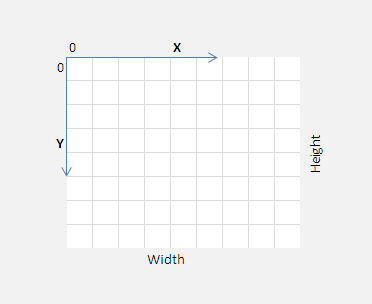
\includegraphics{logos/canvascos}
\end{figure}
\end{frame}

\begin{frame}[fragile]{Wie zeichnet man Vierecke}
\begin{lstlisting}
//um in JS auf das Canvas zuzugreifen
canvas = document.getElementById("game");
context = canvas.getContext("2d");

//gefülltes Viereck
context.fillStyle = color;
context.fillRect(x,y,breite,hoehe);

//ungefülltes mit Rand
context.strokeStyle = color;
context.strokeRect(x, y, breite, höhe);
\end{lstlisting}

\end{frame}

\begin{frame}{Jetzt ihr!}
\begin{itemize}
	\item Fu"gt ein Canvas Element zum HTML-Dokument hinzu
	\item ruft die Funktion Paint game am Ende des Bodys aus dem HTML auf. 
	\item implementiert die Funktion paintGame() 
	\item fügt verschiedene Vierecke dem Canvas Element hinzu. 
\end{itemize}
\end{frame}

\section{Spielbasics}

\begin{frame}{Die Idee - Was wir hier Programmieren wollen}
\begin{figure}[htb]
	\centering
	
\includegraphics[width=1\textwidth]{logos/game}
\end{figure}
\end{frame}

\begin{frame}{Was ist eine Gameloop?}
\begin{itemize}
	\item um das Feld zu aktualsieren wird das Spielfeld nach wenigen Millisekunden neugezeichnet
	\item 
\end{itemize}
\end{frame}

\begin{frame}{start, stop, neustart, clear}
\end{frame}

\section{Der Spieler}

\begin{frame}{Spieler einfügen}
\end{frame}

\begin{frame}{schießen implementieren}
\end{frame}

\section{Die Gegner}
\begin{frame}{Idee zufällige Gegner}
\end{frame}

\begin{frame}{Randomisieren}
\end{frame}

\begin{frame}{Gegner in der Loop hinzufügen}
\end{frame}

\section{Kollisionen}
\begin{frame}{Kollisionen erkennen}
\end{frame}

\begin{frame}{Kollisionen verarbeiten}
\end{frame}

\end{document}
